\documentclass[border=10pt]{standalone}
\usepackage[svgnames]{xcolor}
\usepackage{amsmath}
\usepackage{pgfplots}
\pgfplotsset{compat=newest}
\usepackage[sfdefault]{FiraSans}
\usepackage{FiraMono}
\renewcommand*\familydefault{\sfdefault}
\begin{document}
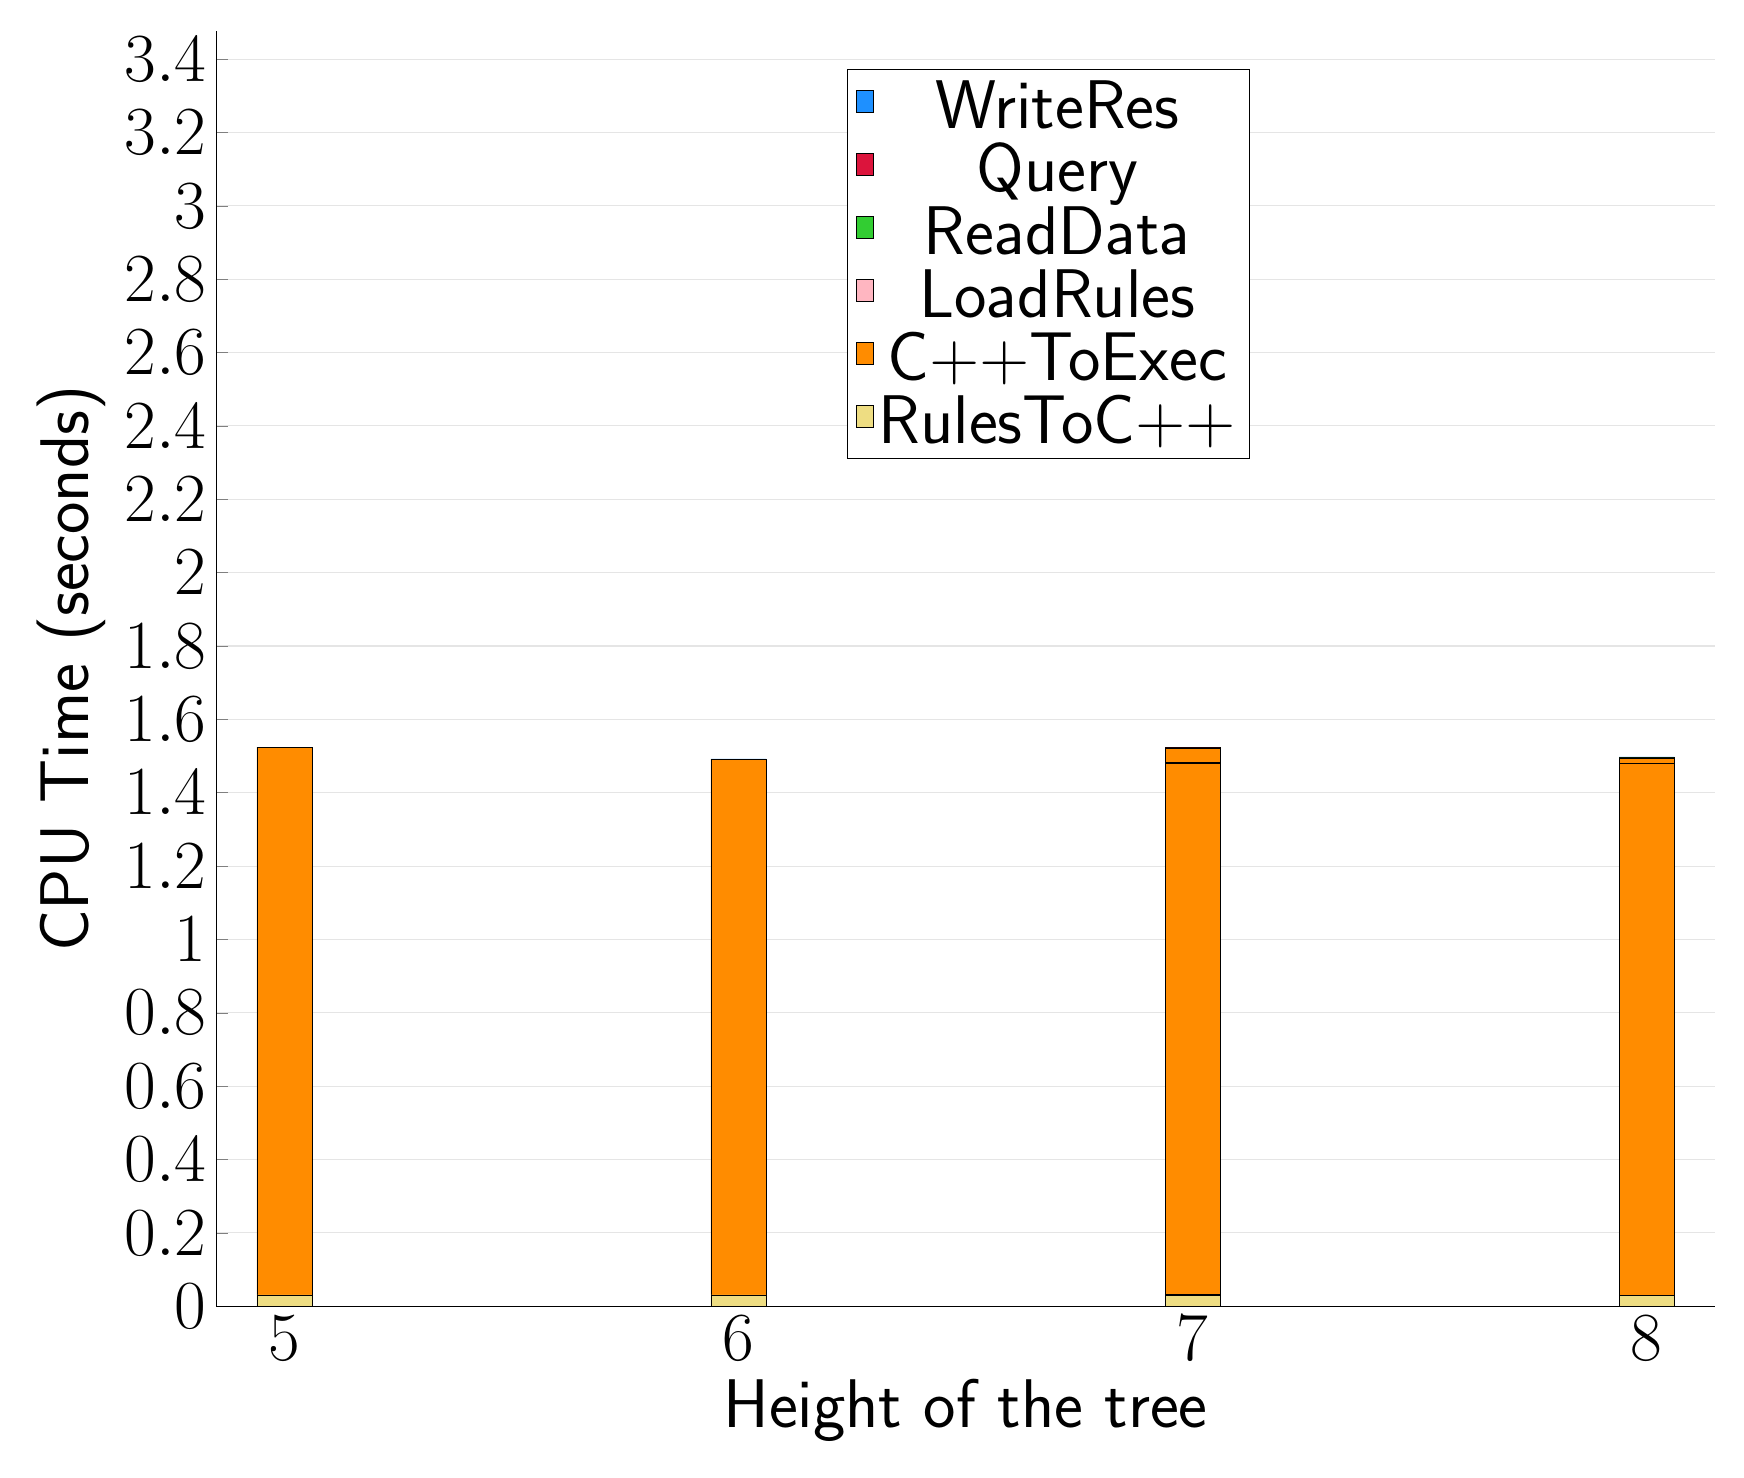
\begin{tikzpicture}
\begin{axis}[
   ybar stacked,
   width=1.7\textwidth,
   bar width=0.7cm,
   ymajorgrids, tick align=inside,
   major grid style={draw=gray!20},
   xtick=data,
   ymin=0, ymax=3.477,
   axis x line*=bottom,
   axis y line*=left,
   enlarge x limits=0.05,
   legend style={
       at={(0.69, 0.97)},
       anchor=north east,
       legend columns=1,
       font=\Huge,
   },
   ylabel={CPU Time (seconds)},
   xlabel={Height of the tree},
   label style={font=\Huge},
   tick label style={font=\Huge},
]
\addlegendimage{fill=DodgerBlue, draw=black, line width=0.2pt}
\addlegendentry{WriteRes}
\addlegendimage{fill=Crimson, draw=black, line width=0.2pt}
\addlegendentry{Query}
\addlegendimage{fill=LimeGreen, draw=black, line width=0.2pt}
\addlegendentry{ReadData}
\addlegendimage{fill=LightPink, draw=black, line width=0.2pt}
\addlegendentry{LoadRules}
\addlegendimage{fill=DarkOrange, draw=black, line width=0.2pt}
\addlegendentry{C++ToExec}
\addlegendimage{fill=LightGoldenrod, draw=black, line width=0.2pt}
\addlegendentry{RulesToC++}
\addplot +[fill=LightGoldenrod, draw=black, line width=0.2pt] coordinates {
(5, 0.031000000000000007)
(6, 0.031000000000000007)
(7, 0.030000000000000006)
(7, 0.030000000000000006)
(7, 0.032999999999999995)
(8, 0.030000000000000006)
(8, 0.030000000000000006)
(8, 0.030000000000000006)
};
\addplot +[fill=DarkOrange, draw=black, line width=0.2pt] coordinates {
(5, 1.492)
(6, 1.4599999999999997)
(7, 1.454)
(7, 1.451)
(7, 1.4880000000000002)
(8, 1.4489999999999998)
(8, 1.464)
(8, 1.449)
};
\addplot +[fill=LightPink, draw=black, line width=0.2pt] coordinates {
(5, 1.3100000000000002e-05)
(6, 0.0)
(7, 0.0)
(7, 0.0)
(7, 0.0)
(8, 0.0)
(8, 1.09e-05)
(8, 0.0)
};
\addplot +[fill=LimeGreen, draw=black, line width=0.2pt] coordinates {
(5, 0.00039299999999999996)
(6, 0.00043950000000000006)
(7, 0.0005379)
(7, 0.0005786999999999999)
(7, 0.0005075)
(8, 0.0008423)
(8, 0.0007861999999999999)
(8, 0.0008617000000000002)
};
\addplot +[fill=Crimson, draw=black, line width=0.2pt] coordinates {
(5, 0.00014810000000000002)
(6, 0.00033820000000000003)
(7, 0.0007549)
(7, 0.0008265)
(7, 0.0007059999999999999)
(8, 0.0019427)
(8, 0.00173)
(8, 0.0019735000000000004)
};
\addplot +[fill=DodgerBlue, draw=black, line width=0.2pt] coordinates {
(5, 0.0003039)
(6, 0.00030809999999999995)
(7, 0.0004587)
(7, 0.0004944)
(7, 0.00044610000000000006)
(8, 0.0009054)
(8, 0.0008553000000000001)
(8, 0.0009327000000000001)
};
\end{axis}
\end{tikzpicture}

\end{document}
